\documentclass{article}

    % Input language encoding
    %\usepackage[utf8]{inputenc}
   
    % Output languages
    %\usepackage[greek, english]{babel}
    % \usepackage{alphabeta}
    
    % Fonts
    %\usepackage[T1,LGR]{fontenc}
    \usepackage{lmodern}

    % Images
    \usepackage{graphicx}
    \usepackage{float}
    \usepackage{caption}
    \usepackage{subcaption}

    % Math
    \usepackage{amsmath}

    % Paragraph Formatting
    \usepackage{parskip}

    % Code
    \usepackage{listings}

        

    \DeclareMathSizes{10}{10}{10}{10}
    \setlength{\parindent}{0cm}

    \title{Part 1.2-2}

\begin{document}

\pagenumbering{gobble}
\date{}
\author{}

\maketitle

In this case, we need to figure out when $ 8 * n^{2} \leq 64* n * \log{n} $.

By plotting it in Matlab, we have the Figure \ref{fig:plot1}:

\begin{figure}
    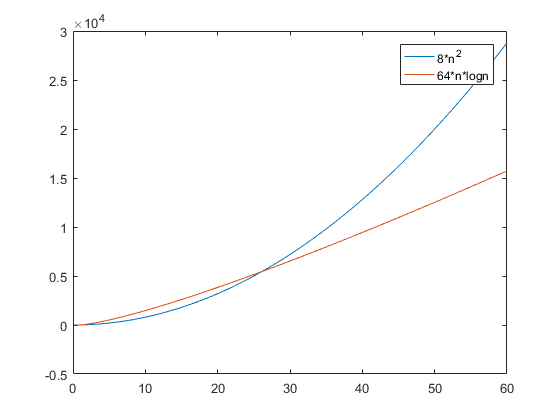
\includegraphics[width=10cm]{1-2-2.png}
    \centering
    \caption{Our plot}
    \label{fig:plot1}
\end{figure}

The Matlab code we used is the following:

\begin{lstlisting}[language=Matlab]
    plot(x,y1,x,y2)
    x = linspace(0,60);
    y1 = 8 * x.^2;
    y2 = 64 * x .* log(x);
    figure();
    plot(x,y1,x,y2);
    legend('8*n^2','64*n*logn');
\end{lstlisting}

As we see the period that $8*n^{2}$ is better than $64*n*\log{n}$ is between 1 and 26, without going into much details in how to find the exact positions. If we want to find them exactly, we could use Numerical Analysis, but our goal here is to just get an overview of how it would look like.
\end{document}